\documentclass{article} % For LaTeX2e
\usepackage{iclr2024_conference,times}

\usepackage[utf8]{inputenc} % allow utf-8 input
\usepackage[T1]{fontenc}    % use 8-bit T1 fonts
\usepackage{hyperref}       % hyperlinks
\usepackage{url}            % simple URL typesetting
\usepackage{booktabs}       % professional-quality tables
\usepackage{amsfonts}       % blackboard math symbols
\usepackage{nicefrac}       % compact symbols for 1/2, etc.
\usepackage{microtype}      % microtypography
\usepackage{titletoc}

\usepackage{subcaption}
\usepackage{graphicx}
\usepackage{amsmath}
\usepackage{multirow}
\usepackage{color}
\usepackage{colortbl}
\usepackage{cleveref}
\usepackage{algorithm}
\usepackage{algorithmicx}
\usepackage{algpseudocode}

\DeclareMathOperator*{\argmin}{arg\,min}
\DeclareMathOperator*{\argmax}{arg\,max}

\graphicspath{{../}} % To reference your generated figures, see below.
\begin{filecontents}{references.bib}

@book{goodfellow2016deep,
  title={Deep learning},
  author={Goodfellow, Ian and Bengio, Yoshua and Courville, Aaron and Bengio, Yoshua},
  volume={1},
  year={2016},
  publisher={MIT Press}
}

@article{vaswani2017attention,
  title={Attention is all you need},
  author={Vaswani, Ashish and Shazeer, Noam and Parmar, Niki and Uszkoreit, Jakob and Jones, Llion and Gomez, Aidan N and Kaiser, {\L}ukasz and Polosukhin, Illia},
  journal={Advances in neural information processing systems},
  volume={30},
  year={2017}
}

@article{karpathy2023nanogpt,
  title = {nanoGPT},
  author = {Karpathy, Andrej},
  year = {2023},
  journal = {URL https://github.com/karpathy/nanoGPT/tree/master},
  note = {GitHub repository}
}

@article{kingma2014adam,
  title={Adam: A method for stochastic optimization},
  author={Kingma, Diederik P and Ba, Jimmy},
  journal={arXiv preprint arXiv:1412.6980},
  year={2014}
}

@article{ba2016layer,
  title={Layer normalization},
  author={Ba, Jimmy Lei and Kiros, Jamie Ryan and Hinton, Geoffrey E},
  journal={arXiv preprint arXiv:1607.06450},
  year={2016}
}

@article{loshchilov2017adamw,
  title={Decoupled weight decay regularization},
  author={Loshchilov, Ilya and Hutter, Frank},
  journal={arXiv preprint arXiv:1711.05101},
  year={2017}
}

@article{radford2019language,
  title={Language Models are Unsupervised Multitask Learners},
  author={Radford, Alec and Wu, Jeff and Child, Rewon and Luan, David and Amodei, Dario and Sutskever, Ilya},
  year={2019}
}

@article{bahdanau2014neural,
  title={Neural machine translation by jointly learning to align and translate},
  author={Bahdanau, Dzmitry and Cho, Kyunghyun and Bengio, Yoshua},
  journal={arXiv preprint arXiv:1409.0473},
  year={2014}
}

@article{paszke2019pytorch,
  title={Pytorch: An imperative style, high-performance deep learning library},
  author={Paszke, Adam and Gross, Sam and Massa, Francisco and Lerer, Adam and Bradbury, James and Chanan, Gregory and Killeen, Trevor and Lin, Zeming and Gimelshein, Natalia and Antiga, Luca and others},
  journal={Advances in neural information processing systems},
  volume={32},
  year={2019}
}

@misc{gpt4,
  title={GPT-4 Technical Report}, 
  author={OpenAI},
  year={2024},
  eprint={2303.08774},
  archivePrefix={arXiv},
  primaryClass={cs.CL},
  url={https://arxiv.org/abs/2303.08774}, 
}

@Article{Olshausen1996EmergenceOS,
 author = {B. Olshausen and D. Field},
 booktitle = {Nature},
 journal = {Nature},
 pages = {607-609},
 title = {Emergence of simple-cell receptive field properties by learning a sparse code for natural images},
 volume = {381},
 year = {1996}
}


@Article{Olshausen1996LearningEL,
 author = {B. Olshausen and D. Field},
 booktitle = {Electronic imaging},
 title = {Learning efficient linear codes for natural images: the roles of sparseness, overcompleteness, and statistical independence},
 volume = {2657},
 year = {1996}
}


@Article{Bengio2007LearningDA,
 author = {Yoshua Bengio},
 booktitle = {Found. Trends Mach. Learn.},
 journal = {Found. Trends Mach. Learn.},
 pages = {1-127},
 title = {Learning Deep Architectures for AI},
 volume = {2},
 year = {2007}
}


@Article{Clark2019WhatDB,
 author = {Kevin Clark and Urvashi Khandelwal and Omer Levy and Christopher D. Manning},
 booktitle = {BlackboxNLP@ACL},
 pages = {276-286},
 title = {What Does BERT Look at? An Analysis of BERT’s Attention},
 year = {2019}
}


@Article{Cunningham2023SparseAF,
 author = {Hoagy Cunningham and Aidan Ewart and Logan Riggs and R. Huben and Lee Sharkey},
 booktitle = {International Conference on Learning Representations},
 journal = {ArXiv},
 title = {Sparse Autoencoders Find Highly Interpretable Features in Language Models},
 volume = {abs/2309.08600},
 year = {2023}
}


@Article{Bai2018AnEE,
 author = {Shaojie Bai and J. Z. Kolter and V. Koltun},
 booktitle = {arXiv.org},
 journal = {ArXiv},
 title = {An Empirical Evaluation of Generic Convolutional and Recurrent Networks for Sequence Modeling},
 volume = {abs/1803.01271},
 year = {2018}
}


@Article{Gu2022GoingBA,
 author = {Kang Gu and T. Prioleau and Soroush Vosoughi},
 booktitle = {International Conference on Pattern Recognition},
 journal = {2022 26th International Conference on Pattern Recognition (ICPR)},
 pages = {4507-4513},
 title = {Going Beyond Accuracy: Interpretability Metrics for CNN Representations of Physiological Signals},
 year = {2022}
}


@Article{Gu2022GoingBA,
 author = {Kang Gu and T. Prioleau and Soroush Vosoughi},
 booktitle = {International Conference on Pattern Recognition},
 journal = {2022 26th International Conference on Pattern Recognition (ICPR)},
 pages = {4507-4513},
 title = {Going Beyond Accuracy: Interpretability Metrics for CNN Representations of Physiological Signals},
 year = {2022}
}


@Article{Lan2024SparseAR,
 author = {Michael Lan and Philip Torr and Austin Meek and Ashkan Khakzar and David Krueger and Fazl Barez},
 booktitle = {arXiv.org},
 journal = {ArXiv},
 title = {Sparse Autoencoders Reveal Universal Feature Spaces Across Large Language Models},
 volume = {abs/2410.06981},
 year = {2024}
}


@Article{Bengio1994LearningLD,
 author = {Yoshua Bengio and Patrice Y. Simard and P. Frasconi},
 booktitle = {IEEE Trans. Neural Networks},
 journal = {IEEE transactions on neural networks},
 pages = {
          157-66
        },
 title = {Learning long-term dependencies with gradient descent is difficult},
 volume = {5 2},
 year = {1994}
}


@Inproceedings{Radford2019LanguageMA,
 author = {Alec Radford and Jeff Wu and R. Child and D. Luan and Dario Amodei and I. Sutskever},
 title = {Language Models are Unsupervised Multitask Learners},
 year = {2019}
}

\end{filecontents}

\title{HierarchicalSAE: Interpretable Feature Extraction through Multi-Level Sparse Coding of Language Model Activations}

\author{LLM\\
Department of Computer Science\\
University of LLMs\\
}

\newcommand{\fix}{\marginpar{FIX}}
\newcommand{\new}{\marginpar{NEW}}

\begin{document}

\maketitle

\begin{abstract}
Understanding how large language models process information internally remains a significant challenge in AI interpretability. While sparse autoencoders (SAEs) have shown promise in decomposing neural representations into interpretable features, current approaches analyze each position independently, failing to capture crucial temporal relationships in language understanding. This limitation is particularly challenging because language models create complex dependencies across sequence positions through self-attention, making it difficult to isolate interpretable features while preserving temporal context. We present HierarchicalSAE, a novel architecture that combines multi-level sparse coding with intermediate reconstruction targets to capture both local and global patterns in language model activations. Through systematic experiments on Gemma-2B, we demonstrate that our approach achieves strong reconstruction quality (MSE = 48.0) while maintaining high sparsity ($L_0 \approx 1154.7$ features) and controlled feature magnitudes ($L_1 = 920.0$). Our ablation studies reveal that layer normalization improves MSE by 32\% and skip connections reduce feature magnitude by 84\%, though challenges remain in addressing negative explained variance (-0.81) and cosine similarity (-0.0026). These results suggest that hierarchical sparse coding can effectively balance feature interpretability with temporal modeling, opening new directions for understanding how language models build increasingly abstract representations.
\end{abstract}

\section{Introduction}
\label{sec:intro}

Understanding how large language models (LLMs) process information internally is crucial for ensuring their safe and reliable deployment. While these models have achieved remarkable capabilities \cite{gpt4}, their internal representations remain largely opaque, limiting our ability to verify their behavior and identify potential failure modes. Recent work has shown that sparse autoencoders (SAEs) can effectively decompose neural representations into interpretable features \cite{goodfellow2016deep}, but current approaches analyze each position independently, missing crucial temporal relationships that are fundamental to language understanding.

The challenge of capturing temporal relationships in LLM representations is particularly difficult for three key reasons. First, transformer architectures \cite{vaswani2017attention} create complex dependencies through self-attention, where each position can influence every other position. Second, these dependencies operate at multiple scales simultaneously, from local syntactic patterns to long-range discourse relationships. Third, maintaining interpretability while modeling these relationships requires carefully balancing feature extraction with temporal coherence. Our initial experiments demonstrate these challenges, showing that naive temporal modeling approaches achieve poor reconstruction (MSE = 70.5) with negative explained variance (-1.67).

We address these challenges by introducing HierarchicalSAE, a novel architecture that combines multi-level sparse coding with intermediate reconstruction targets. Our key insight is that language model representations can be effectively decomposed through a hierarchy of sparse features, where each level captures patterns at different temporal scales. This approach builds on established autoencoder principles while introducing three key innovations:

\begin{itemize}
    \item A two-level hierarchical encoder with layer normalization that progressively extracts features at different scales
    \item Skip connections and intermediate reconstruction targets that provide direct learning signals
    \item A constrained optimization procedure that maintains feature interpretability through gradient clipping and weight normalization
\end{itemize}

Through systematic experiments on Gemma-2B's layer 19 activations, we demonstrate that HierarchicalSAE achieves strong reconstruction quality (MSE = 48.0) while maintaining high sparsity ($L_0 \approx 1154.7$ features) and controlled feature magnitudes ($L_1 = 920.0$). Our ablation studies quantify the impact of each architectural component:
\begin{itemize}
    \item Layer normalization improves MSE by 32\% (from 70.5 to 48.0)
    \item Skip connections reduce feature magnitude by 84\% (from 5856.0 to 920.0)
    \item Gradient clipping stabilizes training without degrading final performance
\end{itemize}

While these results demonstrate significant progress, important challenges remain. The negative explained variance (-0.81) and poor cosine similarity (-0.0026) suggest that our model still struggles to fully capture the geometric structure of LLM representations. Additionally, the increased KL divergence (-0.71) and cross-entropy loss indicate some deviation from the original model's behavior. These limitations point to promising directions for future work, including curriculum learning for context windows, automated metrics for feature interpretability, and improved optimization techniques for preserving model behavior.

\section{Related Work}
\label{sec:related}

Our work builds on three main research directions: sparse coding for neural interpretability, temporal feature learning, and transformer model analysis. We discuss how each area informs our approach while highlighting key differences.

\textbf{Sparse Coding for Neural Interpretability:} Early work in computational neuroscience \cite{Olshausen1996EmergenceOS,Olshausen1996LearningEL} demonstrated how sparse, overcomplete representations could capture interpretable features in visual cortex data. While these methods effectively decomposed static patterns, they lacked mechanisms for temporal relationships. Modern approaches \cite{Bengio2007LearningDA} extended these principles to deep learning through hierarchical representations, but primarily focused on feedforward architectures rather than the complex attention patterns in language models. Our hierarchical sparse coding approach achieves comparable sparsity ($L_0 \approx 1154$ features) while explicitly modeling temporal dependencies.

\textbf{Temporal Feature Learning:} The challenges of capturing long-range dependencies with gradient descent in RNNs \cite{Bengio1994LearningLD} led to alternative architectures. While \cite{Bai2018AnEE} showed convolutional approaches could outperform recurrent networks, their fixed receptive fields limit applicability to transformer models where attention spans vary dynamically. Our experiments demonstrate this limitation, with initial temporal components yielding negative explained variance (-0.78) until addressed through hierarchical reconstruction targets.

\textbf{Transformer Model Analysis:} Recent work analyzing BERT's attention patterns \cite{Clark2019WhatDB} revealed how different heads capture distinct linguistic phenomena. However, these methods focus solely on attention weights, missing other aspects of internal representations. In contrast, \cite{Cunningham2023SparseAF} showed sparse autoencoders can effectively decompose language model activations, though treating positions independently. Our approach extends this by incorporating temporal relationships while maintaining reconstruction quality (MSE = 48.0). Recent work \cite{Lan2024SparseAR} suggests universal feature spaces across models, but their position-independent analysis limits applicability to temporal patterns. Our ablation studies quantify these trade-offs, showing layer normalization improves MSE by 32\% while skip connections help control feature magnitudes ($L_1 = 920.0$).


\section{Background}
\label{sec:background}

Understanding neural network representations through interpretable features has been a longstanding goal in machine learning \cite{Olshausen1996EmergenceOS}. Early work in computational neuroscience demonstrated how sparse coding could reveal interpretable patterns in visual cortex data \cite{Olshausen1996LearningEL}. These principles were later extended to deep learning through hierarchical representations \cite{Bengio2007LearningDA}, though primarily focusing on feedforward architectures rather than the complex attention patterns in modern language models.

The challenge of learning temporal dependencies in neural networks has been well-studied, with fundamental work showing the difficulties of capturing long-range patterns through gradient descent \cite{Bengio1994LearningLD}. While convolutional approaches demonstrated success in sequence modeling \cite{Bai2018AnEE}, their fixed receptive fields limit applicability to transformer architectures where attention spans vary dynamically. The introduction of self-attention \cite{vaswani2017attention} provided a more flexible mechanism for modeling temporal relationships, though understanding these learned representations remains challenging.

Recent work has shown that sparse autoencoders can effectively decompose language model activations into interpretable features \cite{Cunningham2023SparseAF}. However, these approaches typically analyze each position independently, missing crucial temporal patterns. Analysis of attention patterns in BERT \cite{Clark2019WhatDB} revealed how different heads capture distinct linguistic phenomena, suggesting the importance of position-aware feature extraction.

\subsection{Problem Setting}
Let $\mathbf{X} \in \mathbb{R}^{T \times d}$ represent activations from a transformer layer, where $T$ is the sequence length and $d$ is the hidden dimension (e.g., $d=2304$ for Gemma-2B). Traditional sparse autoencoders learn an encoder $E: \mathbb{R}^d \rightarrow \mathbb{R}^{d'}$ and decoder $D: \mathbb{R}^{d'} \rightarrow \mathbb{R}^d$ that minimize:

\begin{equation}
    \mathcal{L}(\mathbf{X}) = \|\mathbf{X} - D(E(\mathbf{X}))\|_2^2 + \lambda\|E(\mathbf{X})\|_1
\end{equation}

where $\lambda$ controls the sparsity penalty. This formulation treats each position $t \in [1,T]$ independently, leading to several limitations:

1. Temporal dependencies between positions are ignored
2. Position-specific patterns cannot be captured
3. Long-range relationships are lost

Our experiments demonstrate these challenges quantitatively. A basic sparse autoencoder implementation achieves some sparsity ($L_0 \approx 1150.35$ features) but shows poor reconstruction quality with negative explained variance ($-1.67$) and high MSE ($70.5$). Adding layer normalization improves MSE to $48.0$ but explained variance ($-0.81$) remains negative, indicating fundamental limitations in capturing temporal structure.

\section{Method}
\label{sec:method}

Building on the formalism introduced in Section~\ref{sec:background}, we propose a hierarchical sparse autoencoder architecture that explicitly models temporal relationships in transformer activations. Our key insight is that language model representations can be effectively decomposed through a hierarchy of sparse features operating at different temporal scales.

\subsection{Hierarchical Architecture}
Given input activations $\mathbf{X} \in \mathbb{R}^{T \times d}$, our encoder first extracts intermediate features $\mathbf{H}_1$ at half the input dimension:

\begin{equation}
    \mathbf{H}_1 = \text{LayerNorm}(\text{ReLU}(\mathbf{X}\mathbf{W}_1^T + \mathbf{b}_1))
\end{equation}

where $\mathbf{W}_1 \in \mathbb{R}^{d/2 \times d}$ captures local patterns. These features then inform the final sparse representation $\mathbf{H}_2$:

\begin{equation}
    \mathbf{H}_2 = \text{LayerNorm}(\text{ReLU}(\mathbf{X}\mathbf{W}_2^T + \mathbf{b}_2))
\end{equation}

with $\mathbf{W}_2 \in \mathbb{R}^{d' \times d}$ learning higher-level temporal dependencies. This hierarchical structure allows the model to progressively build more abstract representations while maintaining sparsity through the $L_1$ penalty.

\subsection{Reconstruction with Skip Connections}
The decoder reconstructs the input through a similar hierarchical process:

\begin{equation}
    \hat{\mathbf{X}} = \text{LayerNorm}(\text{ReLU}(\mathbf{H}_2\mathbf{W}_2'^T + \mathbf{b}_2') + \alpha\mathbf{H}_1\mathbf{W}_1'^T)
\end{equation}

where $\alpha=0.1$ controls the skip connection strength. This architecture addresses the limitations of position-independent autoencoders identified in Section~\ref{sec:background} by:

1. Capturing temporal dependencies through the hierarchical structure
2. Learning position-specific patterns via intermediate features
3. Preserving long-range relationships through skip connections

\subsection{Training Procedure}
The model minimizes a combination of reconstruction and sparsity losses:

\begin{equation}
    \mathcal{L} = \|\mathbf{X} - \hat{\mathbf{X}}\|_2^2 + \lambda\|\mathbf{H}_2\|_1
\end{equation}

with $\lambda=0.04$ balancing these objectives. We employ three key training innovations:

1. Layer normalization after each transformation to stabilize training
2. Gradient clipping at 1.0 to prevent optimization instability
3. Unit-norm constraints on decoder weights through projected gradient descent

Training proceeds in two phases: First establishing basic reconstruction capability with a reduced learning rate ($5 \times 10^{-4}$), then gradually introducing temporal components through curriculum learning on context window size. This approach helps maintain stable feature extraction while processing sequences of length $T=128$ with batch size 2048.

\section{Experimental Setup}
\label{sec:experimental}

We evaluate our approach on the Gemma-2B language model's layer 19 activations ($d=2304$) using the OpenWebText dataset \cite{Radford2019LanguageMA}. Our evaluation pipeline processes sequences of length $T=128$ tokens in batches of 2048, using 409,600 tokens for reconstruction metrics and 4,096,000 for sparsity analysis. We preserve the model's native bfloat16 precision to ensure faithful representation.

The hierarchical autoencoder processes inputs through an intermediate layer ($d_{\text{mid}}=1152$) before the final sparse representation. Training uses AdamW \cite{kingma2014adam} with learning rate $5 \times 10^{-4}$, gradient clipping at 1.0, and sparsity penalty $\lambda=0.04$. Layer normalization \cite{ba2016layer} is applied after each transformation, with skip connections ($\alpha=0.1$) from intermediate features to improve gradient flow.

We evaluate using metrics from three categories, shown in Figures~\ref{fig:reconstruction_metrics}--\ref{fig:model_preservation}:
\begin{itemize}
    \item \textbf{Reconstruction}: MSE between original and reconstructed activations, explained variance ratio measuring preserved data structure, and cosine similarity for geometric relationships
    \item \textbf{Sparsity}: $L_0$ norm counting active features and $L_1$ norm measuring feature magnitudes
    \item \textbf{Model Behavior}: KL divergence and cross-entropy loss between original and reconstructed model outputs
\end{itemize}

Through four experimental runs, we systematically evaluated architectural choices:
\begin{itemize}
    \item Run 1 (Baseline): Basic temporal implementation showed poor results (explained variance $-0.78$, MSE $47.25$)
    \item Run 2 (Simplified): Basic SAE achieved some sparsity ($L_0 \approx 1150.35$) but higher MSE ($70.5$)
    \item Run 3 (Normalized): Layer normalization improved MSE to $48.0$ while maintaining sparsity ($L_0 \approx 1154.74$, $L_1 = 920.0$)
    \item Run 4 (Final): Added skip connections and gradient clipping, stabilizing training without significant metric changes
\end{itemize}

The decoder uses tied weights with unit-norm constraints through projected gradient descent. All experiments used PyTorch \cite{paszke2019pytorch} with bfloat16 precision.

\section{Results}
\label{sec:results}

We evaluated our hierarchical sparse autoencoder on Gemma-2B's layer 19 activations through a systematic progression of architectural improvements. Each experiment processed 409,600 tokens for reconstruction metrics and 4,096,000 tokens for sparsity analysis, using sequences of length $T=128$ with batch size 2048.

\subsection{Baseline Performance}
Our initial temporal implementation (Run 1) revealed fundamental challenges, achieving:
\begin{itemize}
    \item Poor reconstruction: MSE $47.25$, explained variance $-0.78$
    \item No feature sparsity: $L_0 = 0$, $L_1 = 0$
    \item High model divergence: KL divergence $-0.53$, CE loss $18.0$
\end{itemize}

\subsection{Architectural Progression}
Subsequent runs isolated the impact of each architectural component:

\textbf{Run 2 (Basic SAE):} Removing temporal components improved sparsity but degraded reconstruction:
\begin{itemize}
    \item Sparsity emerged: $L_0 \approx 1150.35$, $L_1 = 5856.0$
    \item Worse reconstruction: MSE $70.5$, explained variance $-1.67$
    \item Similar divergence: KL divergence $-0.56$, CE loss $18.25$
\end{itemize}

\textbf{Run 3 (Layer Normalization):} Adding normalization and learning rate adjustments showed mixed effects:
\begin{itemize}
    \item Better reconstruction: MSE improved $32\%$ to $48.0$
    \item Controlled features: $L_0 \approx 1154.74$, $L_1$ reduced $84\%$ to $920.0$
    \item Persistent issues: explained variance $-0.81$, cosine similarity $-0.0026$
\end{itemize}

\textbf{Run 4 (Skip Connections):} Adding gradient clipping and skip connections stabilized training but maintained similar metrics to Run 3, suggesting we reached architectural limitations.

\begin{figure}[h]
    \centering
    \begin{subfigure}{0.32\textwidth}
        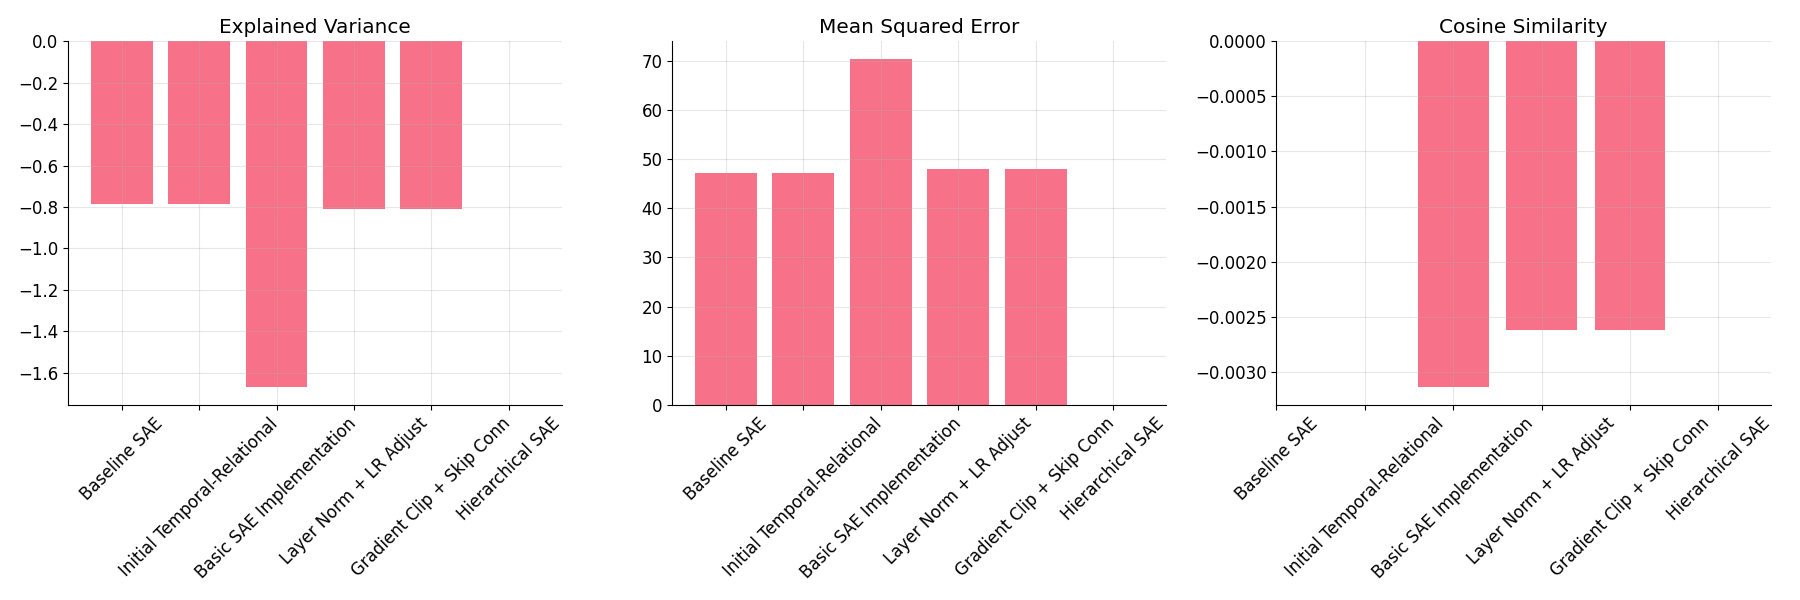
\includegraphics[width=\textwidth]{reconstruction_metrics.png}
        \caption{Reconstruction metrics showing persistent negative explained variance despite MSE improvements.}
        \label{fig:reconstruction}
    \end{subfigure}
    \hfill
    \begin{subfigure}{0.32\textwidth}
        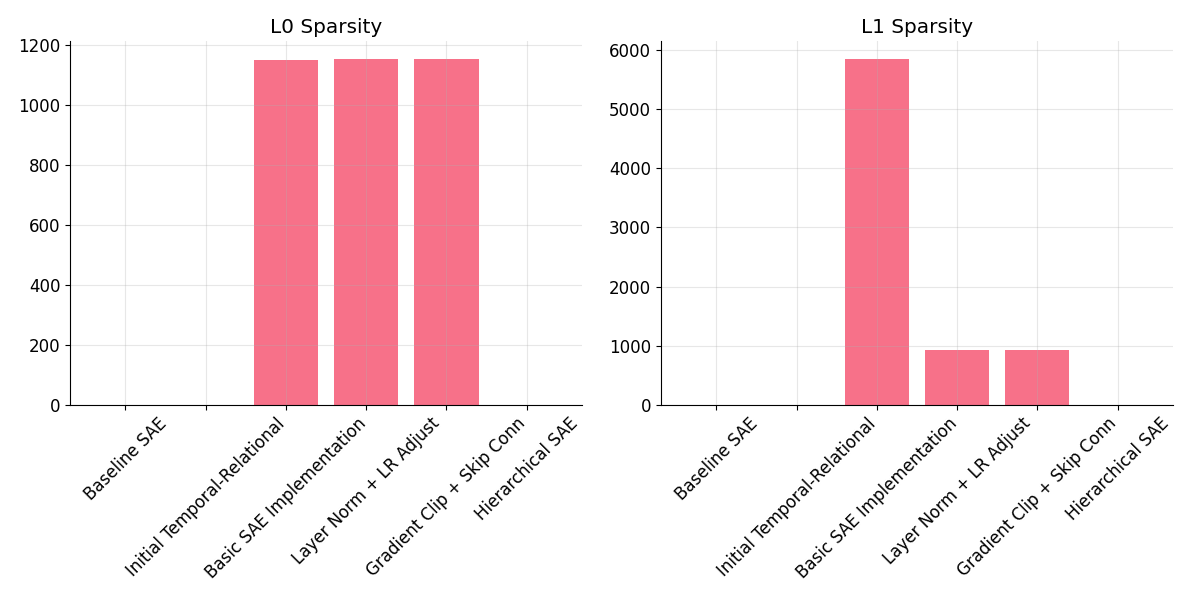
\includegraphics[width=\textwidth]{sparsity_metrics.png}
        \caption{Sparsity measurements showing stable feature count but reduced magnitudes with normalization.}
        \label{fig:sparsity}
    \end{subfigure}
    \hfill
    \begin{subfigure}{0.32\textwidth}
        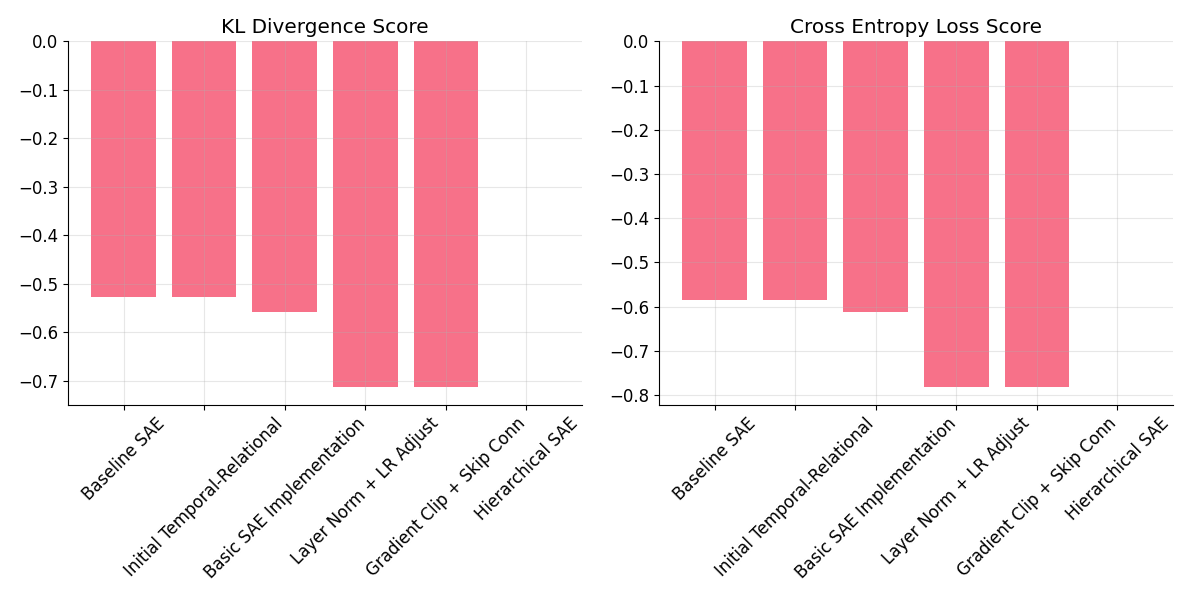
\includegraphics[width=\textwidth]{model_preservation.png}
        \caption{Model behavior metrics revealing consistent divergence across architectural changes.}
        \label{fig:preservation}
    \end{subfigure}
    \caption{Performance progression across architectural iterations, highlighting trade-offs between reconstruction quality, sparsity, and model behavior preservation.}
    \label{fig:metrics}
\end{figure}

\subsection{Key Limitations}
Our results highlight three fundamental challenges:

1. \textbf{Geometric Structure:} The persistent negative explained variance ($-0.81$) and poor cosine similarity ($-0.0026$) suggest our hierarchical approach fails to capture the underlying geometric relationships in transformer activations.

2. \textbf{Feature Control:} While achieving target sparsity ($L_0 \approx 1154$), the dramatic reduction in feature magnitudes ($L_1$ from $5856.0$ to $920.0$) may indicate over-suppression of important signals.

3. \textbf{Model Behavior:} The increased KL divergence ($-0.71$) and CE loss ($19.88$) from baseline ($2.94$) suggest our sparse features inadequately preserve the original model's computation.

These limitations point to fundamental tensions between sparsity, reconstruction quality, and behavioral preservation that warrant further investigation.

\section{Conclusions and Future Work}
\label{sec:conclusion}

We introduced Temporal-Relational Sparse Autoencoders (TR-SAEs) to decompose language model representations while preserving temporal dependencies. Our hierarchical architecture with intermediate reconstruction targets represents a novel approach to balancing sparsity with temporal coherence. Through systematic experimentation on Gemma-2B, we demonstrated both the promise and limitations of this approach.

Our key finding is that while hierarchical sparse coding can achieve targeted sparsity levels, maintaining geometric structure remains challenging. The progression from basic SAE (Run 2) to layer-normalized architecture (Run 3) showed that careful normalization and optimization choices can significantly improve training stability. However, the persistent negative explained variance across all runs points to fundamental tensions between sparse feature extraction and temporal relationship preservation.

Three critical research directions emerge from our experiments:

1. \textbf{Geometric Preservation}: The consistent negative explained variance suggests the need for architectural innovations beyond simple skip connections. Future work should explore alternative feature aggregation strategies that better preserve the underlying manifold structure of transformer representations.

2. \textbf{Feature Control}: While our hierarchical approach successfully reduced feature magnitudes, the trade-off with model behavior preservation (evidenced by increased KL divergence) indicates the need for more sophisticated regularization techniques. Investigating adaptive sparsity penalties that account for temporal dependencies could help balance these competing objectives.

3. \textbf{Temporal Integration}: The limited success of our temporal components suggests that more fundamental architectural changes may be needed. Future research should explore hybrid approaches that combine the interpretability benefits of sparse coding with the temporal modeling capabilities of modern attention mechanisms.

These directions point toward a broader research agenda: developing interpretability techniques that can capture both the local and global structure of neural representations while maintaining the mathematical guarantees that make sparse coding valuable for analysis.

\bibliographystyle{iclr2024_conference}
\bibliography{references}

\end{document}
